% Options for packages loaded elsewhere
\PassOptionsToPackage{unicode}{hyperref}
\PassOptionsToPackage{hyphens}{url}
%
\documentclass[
]{article}
\usepackage{lmodern}
\usepackage{amssymb,amsmath}
\usepackage{ifxetex,ifluatex}
\ifnum 0\ifxetex 1\fi\ifluatex 1\fi=0 % if pdftex
  \usepackage[T1]{fontenc}
  \usepackage[utf8]{inputenc}
  \usepackage{textcomp} % provide euro and other symbols
\else % if luatex or xetex
  \usepackage{unicode-math}
  \defaultfontfeatures{Scale=MatchLowercase}
  \defaultfontfeatures[\rmfamily]{Ligatures=TeX,Scale=1}
\fi
% Use upquote if available, for straight quotes in verbatim environments
\IfFileExists{upquote.sty}{\usepackage{upquote}}{}
\IfFileExists{microtype.sty}{% use microtype if available
  \usepackage[]{microtype}
  \UseMicrotypeSet[protrusion]{basicmath} % disable protrusion for tt fonts
}{}
\makeatletter
\@ifundefined{KOMAClassName}{% if non-KOMA class
  \IfFileExists{parskip.sty}{%
    \usepackage{parskip}
  }{% else
    \setlength{\parindent}{0pt}
    \setlength{\parskip}{6pt plus 2pt minus 1pt}}
}{% if KOMA class
  \KOMAoptions{parskip=half}}
\makeatother
\usepackage{xcolor}
\IfFileExists{xurl.sty}{\usepackage{xurl}}{} % add URL line breaks if available
\IfFileExists{bookmark.sty}{\usepackage{bookmark}}{\usepackage{hyperref}}
\hypersetup{
  pdftitle={Analysis},
  pdfauthor={Nathan Green},
  hidelinks,
  pdfcreator={LaTeX via pandoc}}
\urlstyle{same} % disable monospaced font for URLs
\usepackage[margin=1in]{geometry}
\usepackage{color}
\usepackage{fancyvrb}
\newcommand{\VerbBar}{|}
\newcommand{\VERB}{\Verb[commandchars=\\\{\}]}
\DefineVerbatimEnvironment{Highlighting}{Verbatim}{commandchars=\\\{\}}
% Add ',fontsize=\small' for more characters per line
\usepackage{framed}
\definecolor{shadecolor}{RGB}{248,248,248}
\newenvironment{Shaded}{\begin{snugshade}}{\end{snugshade}}
\newcommand{\AlertTok}[1]{\textcolor[rgb]{0.94,0.16,0.16}{#1}}
\newcommand{\AnnotationTok}[1]{\textcolor[rgb]{0.56,0.35,0.01}{\textbf{\textit{#1}}}}
\newcommand{\AttributeTok}[1]{\textcolor[rgb]{0.77,0.63,0.00}{#1}}
\newcommand{\BaseNTok}[1]{\textcolor[rgb]{0.00,0.00,0.81}{#1}}
\newcommand{\BuiltInTok}[1]{#1}
\newcommand{\CharTok}[1]{\textcolor[rgb]{0.31,0.60,0.02}{#1}}
\newcommand{\CommentTok}[1]{\textcolor[rgb]{0.56,0.35,0.01}{\textit{#1}}}
\newcommand{\CommentVarTok}[1]{\textcolor[rgb]{0.56,0.35,0.01}{\textbf{\textit{#1}}}}
\newcommand{\ConstantTok}[1]{\textcolor[rgb]{0.00,0.00,0.00}{#1}}
\newcommand{\ControlFlowTok}[1]{\textcolor[rgb]{0.13,0.29,0.53}{\textbf{#1}}}
\newcommand{\DataTypeTok}[1]{\textcolor[rgb]{0.13,0.29,0.53}{#1}}
\newcommand{\DecValTok}[1]{\textcolor[rgb]{0.00,0.00,0.81}{#1}}
\newcommand{\DocumentationTok}[1]{\textcolor[rgb]{0.56,0.35,0.01}{\textbf{\textit{#1}}}}
\newcommand{\ErrorTok}[1]{\textcolor[rgb]{0.64,0.00,0.00}{\textbf{#1}}}
\newcommand{\ExtensionTok}[1]{#1}
\newcommand{\FloatTok}[1]{\textcolor[rgb]{0.00,0.00,0.81}{#1}}
\newcommand{\FunctionTok}[1]{\textcolor[rgb]{0.00,0.00,0.00}{#1}}
\newcommand{\ImportTok}[1]{#1}
\newcommand{\InformationTok}[1]{\textcolor[rgb]{0.56,0.35,0.01}{\textbf{\textit{#1}}}}
\newcommand{\KeywordTok}[1]{\textcolor[rgb]{0.13,0.29,0.53}{\textbf{#1}}}
\newcommand{\NormalTok}[1]{#1}
\newcommand{\OperatorTok}[1]{\textcolor[rgb]{0.81,0.36,0.00}{\textbf{#1}}}
\newcommand{\OtherTok}[1]{\textcolor[rgb]{0.56,0.35,0.01}{#1}}
\newcommand{\PreprocessorTok}[1]{\textcolor[rgb]{0.56,0.35,0.01}{\textit{#1}}}
\newcommand{\RegionMarkerTok}[1]{#1}
\newcommand{\SpecialCharTok}[1]{\textcolor[rgb]{0.00,0.00,0.00}{#1}}
\newcommand{\SpecialStringTok}[1]{\textcolor[rgb]{0.31,0.60,0.02}{#1}}
\newcommand{\StringTok}[1]{\textcolor[rgb]{0.31,0.60,0.02}{#1}}
\newcommand{\VariableTok}[1]{\textcolor[rgb]{0.00,0.00,0.00}{#1}}
\newcommand{\VerbatimStringTok}[1]{\textcolor[rgb]{0.31,0.60,0.02}{#1}}
\newcommand{\WarningTok}[1]{\textcolor[rgb]{0.56,0.35,0.01}{\textbf{\textit{#1}}}}
\usepackage{graphicx,grffile}
\makeatletter
\def\maxwidth{\ifdim\Gin@nat@width>\linewidth\linewidth\else\Gin@nat@width\fi}
\def\maxheight{\ifdim\Gin@nat@height>\textheight\textheight\else\Gin@nat@height\fi}
\makeatother
% Scale images if necessary, so that they will not overflow the page
% margins by default, and it is still possible to overwrite the defaults
% using explicit options in \includegraphics[width, height, ...]{}
\setkeys{Gin}{width=\maxwidth,height=\maxheight,keepaspectratio}
% Set default figure placement to htbp
\makeatletter
\def\fps@figure{htbp}
\makeatother
\setlength{\emergencystretch}{3em} % prevent overfull lines
\providecommand{\tightlist}{%
  \setlength{\itemsep}{0pt}\setlength{\parskip}{0pt}}
\setcounter{secnumdepth}{5}

\title{Analysis}
\author{Nathan Green}
\date{17/03/2020}

\begin{document}
\maketitle

The raw annual risk of death is calculated by the proportion of people
in each age, sex, ethnicity group who die each year (with those who
emigrate being censored, of course). Separate survivorship curve for
each year of birth, as life expectancy changes over time. There is sex
differences; ethnicity doesn't make much of a difference.

ETHPOP is based on ONS data in what year?

\begin{Shaded}
\begin{Highlighting}[]
\KeywordTok{library}\NormalTok{(readr)}
\KeywordTok{library}\NormalTok{(purrr)}
\KeywordTok{library}\NormalTok{(dplyr)}
\KeywordTok{library}\NormalTok{(ggplot2)}
\KeywordTok{library}\NormalTok{(scales)}
\KeywordTok{library}\NormalTok{(reshape2)}
\KeywordTok{library}\NormalTok{(survivorETHPOP)}
\end{Highlighting}
\end{Shaded}

\hypertarget{ethpop}{%
\section{ETHPOP}\label{ethpop}}

We want to compare between the ONS mortality statistics and ETHPOP. From
\href{https://www.ons.gov.uk/peoplepopulationandcommunity/healthandsocialcare/healthandlifeexpectancies/methodologies/guidetocalculatingnationallifetables}{here}
it details their method. They calculate a \emph{central rate of
mortality} as the average across 3 years. \[
m_x = \sum_{y1,y2,y3} deaths_i/ \sum_{y1,y2,y3} pop_i
\]

Finally, they calculate the \emph{mortality rate} which is what we will
be using to compare and is equivalent to the hazard. \[
q_x = 2 m_x/(2 + m_x)
\]

\hypertarget{individual-categories-hazards-and-survival}{%
\subsection{Individual categories hazards and
survival}\label{individual-categories-hazards-and-survival}}

\begin{Shaded}
\begin{Highlighting}[]
\NormalTok{ETHPOP_lifetable <-}\StringTok{ }\KeywordTok{make_ETHPOP_lifetable}\NormalTok{()}
\CommentTok{# save(ETHPOP_lifetable, file = here::here("data", "ETHPOP_lifetable.RData"))}


\KeywordTok{head}\NormalTok{(ETHPOP_lifetable)}
\end{Highlighting}
\end{Shaded}

\begin{verbatim}
FALSE # A tibble: 6 x 16
FALSE   ETH.group   age sex   deaths  year    pop    id yr_age death_rate      mx      qx     Lx      Tx    ex     S  S_qx
FALSE   <chr>     <dbl> <chr>  <dbl> <dbl>  <dbl> <int> <chr>       <dbl>   <dbl>   <dbl>  <dbl>   <dbl> <dbl> <dbl> <dbl>
FALSE 1 BAN           0 F       9.37  2011  4844.   101 2011_0    0.00193 0.00193 0.00193  4826. 243722.  50.3 0.998 0.998
FALSE 2 BAN           0 M      10.7   2011  4884.   101 2011_0    0.00219 0.00219 0.00219  4849. 250641.  51.3 0.998 0.998
FALSE 3 BLA           0 F      16.4   2011 10529.   101 2011_0    0.00156 0.00156 0.00156 10686. 711828.  67.6 0.998 0.998
FALSE 4 BLA           0 M      19.2   2011 10806.   101 2011_0    0.00178 0.00178 0.00178 10889. 777737.  72.0 0.998 0.998
FALSE 5 BLC           0 F       4.91  2011  2728.   101 2011_0    0.00180 0.00180 0.00180  2681. 147650.  54.1 0.998 0.998
FALSE 6 BLC           0 M       5.25  2011  2736.   101 2011_0    0.00192 0.00192 0.00192  2673. 149569.  54.7 0.998 0.998
\end{verbatim}

\begin{Shaded}
\begin{Highlighting}[]
\NormalTok{ETHPOP_lifetable }\OperatorTok\StringTok{ }
\StringTok{  }\KeywordTok{survivor_curve}\NormalTok{(}\DataTypeTok{group =} \KeywordTok{list}\NormalTok{(}\DataTypeTok{sex =} \StringTok{"M"}\NormalTok{,}
                              \DataTypeTok{ETH.group =} \StringTok{"WHO"}\NormalTok{,}
                              \DataTypeTok{year =} \DecValTok{2011}\NormalTok{)) }\OperatorTok\StringTok{ }
\StringTok{  }\KeywordTok{haz_plot}\NormalTok{()}

\NormalTok{ETHPOP_lifetable }\OperatorTok\StringTok{ }
\StringTok{  }\KeywordTok{survivor_curve}\NormalTok{(}\DataTypeTok{group =} \KeywordTok{list}\NormalTok{(}\DataTypeTok{sex =} \StringTok{"M"}\NormalTok{,}
                              \DataTypeTok{ETH.group =} \StringTok{"WHO"}\NormalTok{,}
                              \DataTypeTok{year =} \DecValTok{2049}\NormalTok{)) }\OperatorTok\StringTok{ }
\StringTok{  }\KeywordTok{haz_plot}\NormalTok{(}\DataTypeTok{add =} \OtherTok{TRUE}\NormalTok{)}
\end{Highlighting}
\end{Shaded}

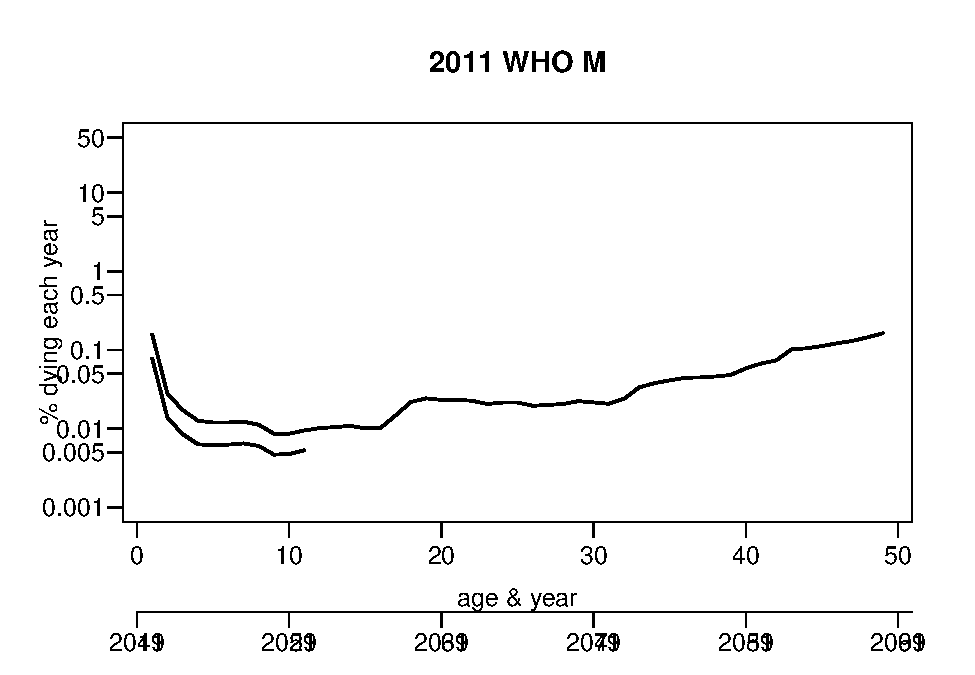
\includegraphics{C:/Users/Nathan/Documents/R/survivorETHPOP/docs/analysis_files/figure-latex/unnamed-chunk-2-1.pdf}

\begin{Shaded}
\begin{Highlighting}[]
\NormalTok{ETHPOP_lifetable }\OperatorTok\StringTok{ }
\StringTok{  }\KeywordTok{survivor_curve}\NormalTok{(}\DataTypeTok{group =} \KeywordTok{list}\NormalTok{(}\DataTypeTok{sex =} \StringTok{"M"}\NormalTok{,}
                              \DataTypeTok{ETH.group =} \StringTok{"WHO"}\NormalTok{,}
                              \DataTypeTok{year =} \DecValTok{2011}\NormalTok{)) }\OperatorTok
\StringTok{  }\KeywordTok{haz_plot}\NormalTok{()}

\ControlFlowTok{for}\NormalTok{ (i }\ControlFlowTok{in} \DecValTok{2012}\OperatorTok{:}\DecValTok{2043}\NormalTok{) \{}
\NormalTok{  ETHPOP_lifetable }\OperatorTok\StringTok{ }
\StringTok{    }\KeywordTok{survivor_curve}\NormalTok{(}\DataTypeTok{group =} \KeywordTok{list}\NormalTok{(}\DataTypeTok{sex =} \StringTok{"M"}\NormalTok{,}
                                \DataTypeTok{ETH.group =} \StringTok{"WHO"}\NormalTok{,}
                                \DataTypeTok{year =}\NormalTok{ i)) }\OperatorTok\StringTok{ }
\StringTok{    }\KeywordTok{haz_plot}\NormalTok{(}\DataTypeTok{add =} \OtherTok{TRUE}\NormalTok{)}
\NormalTok{\}}
\end{Highlighting}
\end{Shaded}

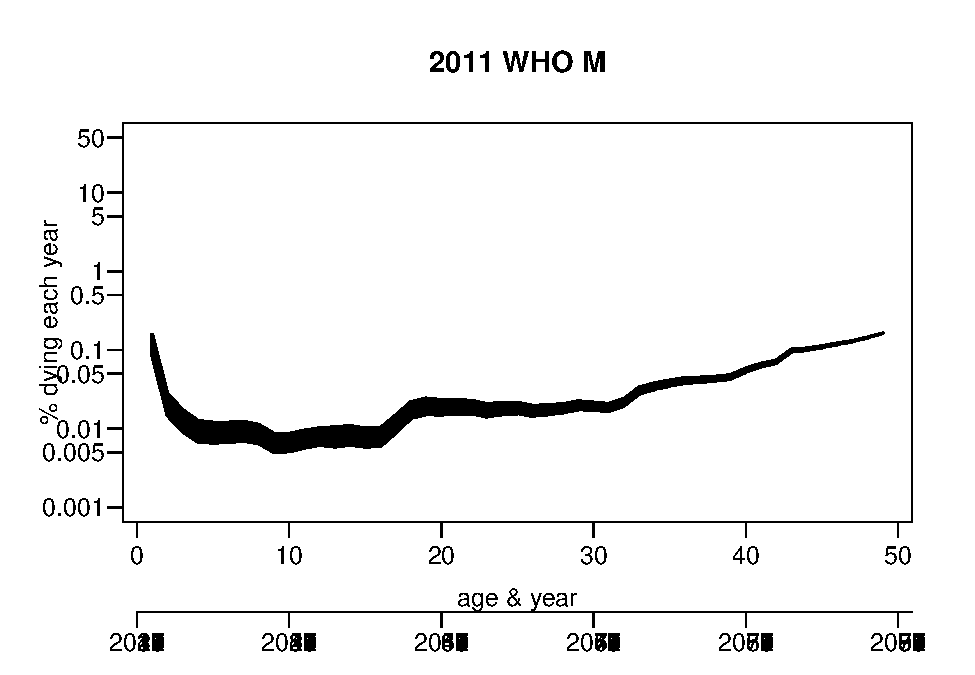
\includegraphics{C:/Users/Nathan/Documents/R/survivorETHPOP/docs/analysis_files/figure-latex/unnamed-chunk-2-2.pdf}

\begin{Shaded}
\begin{Highlighting}[]
\KeywordTok{par}\NormalTok{(}\DataTypeTok{mfrow=}\KeywordTok{c}\NormalTok{(}\DecValTok{1}\NormalTok{,}\DecValTok{2}\NormalTok{))}
\NormalTok{dat <-}\StringTok{ }\NormalTok{ETHPOP_lifetable }\OperatorTok\StringTok{ }
\StringTok{  }\KeywordTok{survivor_curve}\NormalTok{(}\DataTypeTok{group =} \KeywordTok{list}\NormalTok{(}\DataTypeTok{sex =} \StringTok{"M"}\NormalTok{,}
                              \DataTypeTok{ETH.group =} \StringTok{"BAN"}\NormalTok{,}
                              \DataTypeTok{year =} \DecValTok{2011}\NormalTok{)) }\OperatorTok\StringTok{ }
\StringTok{  }\KeywordTok{haz_plot}\NormalTok{() }\OperatorTok\StringTok{ }
\StringTok{  }\KeywordTok{surv_plot}\NormalTok{()}
\end{Highlighting}
\end{Shaded}

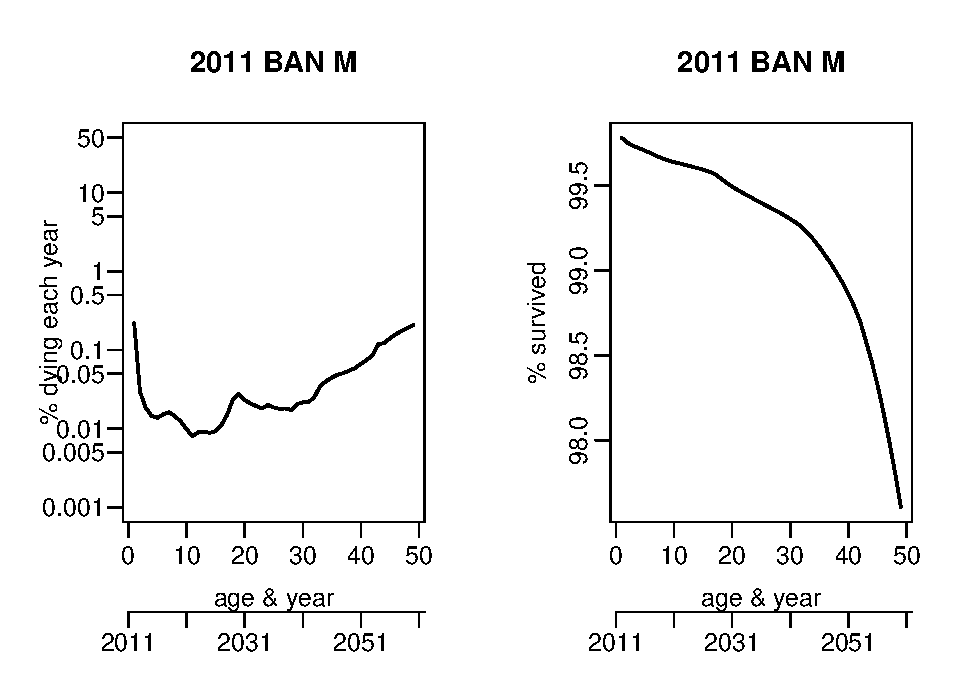
\includegraphics{C:/Users/Nathan/Documents/R/survivorETHPOP/docs/analysis_files/figure-latex/unnamed-chunk-2-3.pdf}

\hypertarget{ethnic-groups}{%
\subsubsection{Ethnic groups}\label{ethnic-groups}}

\begin{Shaded}
\begin{Highlighting}[]
\NormalTok{ethnic_grps <-}\StringTok{ }\KeywordTok{c}\NormalTok{(}\StringTok{"BAN"}\NormalTok{, }\StringTok{"BLA"}\NormalTok{, }\StringTok{"BLC"}\NormalTok{, }\StringTok{"CHI"}\NormalTok{, }\StringTok{"IND"}\NormalTok{, }\StringTok{"MIX"}\NormalTok{,}
                 \StringTok{"OAS"}\NormalTok{, }\StringTok{"OBL"}\NormalTok{, }\StringTok{"OTH"}\NormalTok{, }\StringTok{"PAK"}\NormalTok{, }\StringTok{"WBI"}\NormalTok{, }\StringTok{"WHO"}\NormalTok{)}

\NormalTok{ETHPOP_lifetable }\OperatorTok\StringTok{ }
\StringTok{  }\KeywordTok{survivor_curve}\NormalTok{(}\DataTypeTok{group =} \KeywordTok{list}\NormalTok{(}\DataTypeTok{sex =} \StringTok{"M"}\NormalTok{,}
                              \DataTypeTok{ETH.group =} \StringTok{"BAN"}\NormalTok{,}
                              \DataTypeTok{year =} \DecValTok{2011}\NormalTok{)) }\OperatorTok\StringTok{ }
\StringTok{  }\KeywordTok{haz_plot}\NormalTok{()}

\ControlFlowTok{for}\NormalTok{ (i }\ControlFlowTok{in}\NormalTok{ ethnic_grps) \{}
\NormalTok{  ETHPOP_lifetable }\OperatorTok\StringTok{ }
\StringTok{    }\KeywordTok{survivor_curve}\NormalTok{(}\DataTypeTok{group =} \KeywordTok{list}\NormalTok{(}\DataTypeTok{sex =} \StringTok{"M"}\NormalTok{,}
                                \DataTypeTok{ETH.group =}\NormalTok{ i,}
                                \DataTypeTok{year =} \DecValTok{2011}\NormalTok{)) }\OperatorTok\StringTok{ }
\StringTok{    }\KeywordTok{haz_plot}\NormalTok{(}\DataTypeTok{add =} \OtherTok{TRUE}\NormalTok{)}
\NormalTok{\}}
\end{Highlighting}
\end{Shaded}

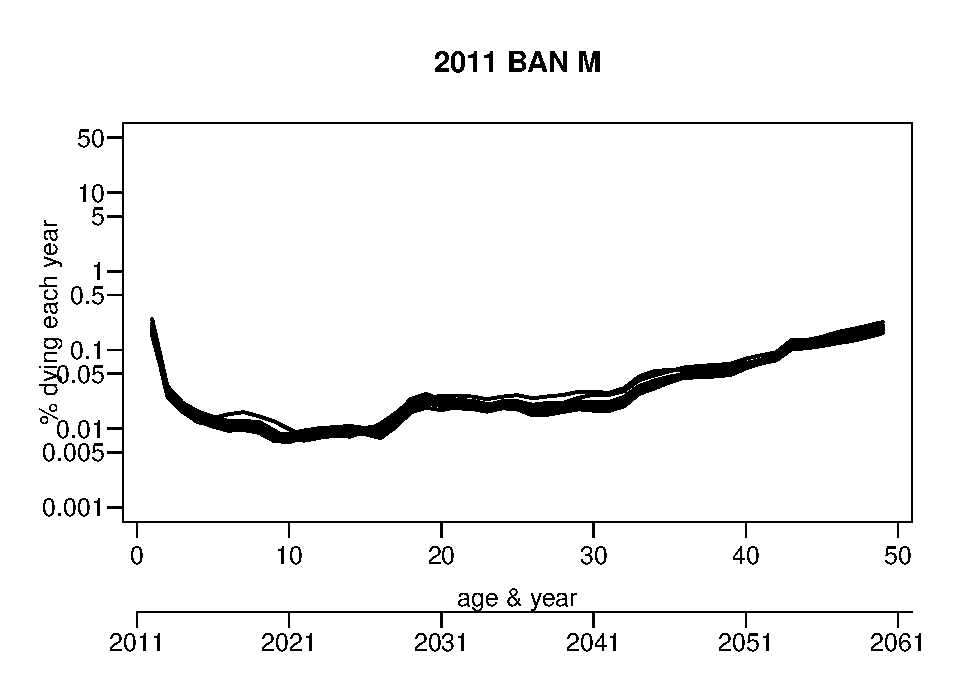
\includegraphics{C:/Users/Nathan/Documents/R/survivorETHPOP/docs/analysis_files/figure-latex/unnamed-chunk-3-1.pdf}

\begin{Shaded}
\begin{Highlighting}[]
\NormalTok{baseyr_}\DecValTok{2011}\NormalTok{ <-}\StringTok{ }\NormalTok{ETHPOP_lifetable}\OperatorTok{$}\NormalTok{id[ETHPOP_lifetable}\OperatorTok{$}\NormalTok{yr_age }\OperatorTok{==}\StringTok{ "2011_0"}\NormalTok{][}\DecValTok{1}\NormalTok{]}

\NormalTok{ETHPOP_lifetable_2011M <-}\StringTok{ }\NormalTok{ETHPOP_lifetable }\OperatorTok\StringTok{ }
\StringTok{  }\KeywordTok{filter}\NormalTok{(id }\OperatorTok{==}\StringTok{ }\NormalTok{baseyr_}\DecValTok{2011}\NormalTok{,}
\NormalTok{         sex }\OperatorTok{==}\StringTok{ "M"}\NormalTok{)}

\NormalTok{ETHPOP_lifetable_2011F <-}\StringTok{ }\NormalTok{ETHPOP_lifetable }\OperatorTok\StringTok{ }
\StringTok{  }\KeywordTok{filter}\NormalTok{(id }\OperatorTok{==}\StringTok{ }\NormalTok{baseyr_}\DecValTok{2011}\NormalTok{,}
\NormalTok{         sex }\OperatorTok{==}\StringTok{ "F"}\NormalTok{)}
\end{Highlighting}
\end{Shaded}

\begin{Shaded}
\begin{Highlighting}[]
\CommentTok{## ggplot}

\KeywordTok{ggplot}\NormalTok{(ETHPOP_lifetable_2011M, }\KeywordTok{aes}\NormalTok{(}\DataTypeTok{x =}\NormalTok{ age, }\DataTypeTok{y =}\NormalTok{ death_rate, }\DataTypeTok{colour =}\NormalTok{ ETH.group)) }\OperatorTok{+}
\StringTok{  }\KeywordTok{geom_line}\NormalTok{() }\OperatorTok{+}
\StringTok{  }\CommentTok{# scale_y_continuous(trans='log2') +}
\StringTok{  }\KeywordTok{coord_trans}\NormalTok{(}\DataTypeTok{y =} \StringTok{"log10"}\NormalTok{) }\OperatorTok{+}
\StringTok{  }\KeywordTok{theme_bw}\NormalTok{()}
\end{Highlighting}
\end{Shaded}

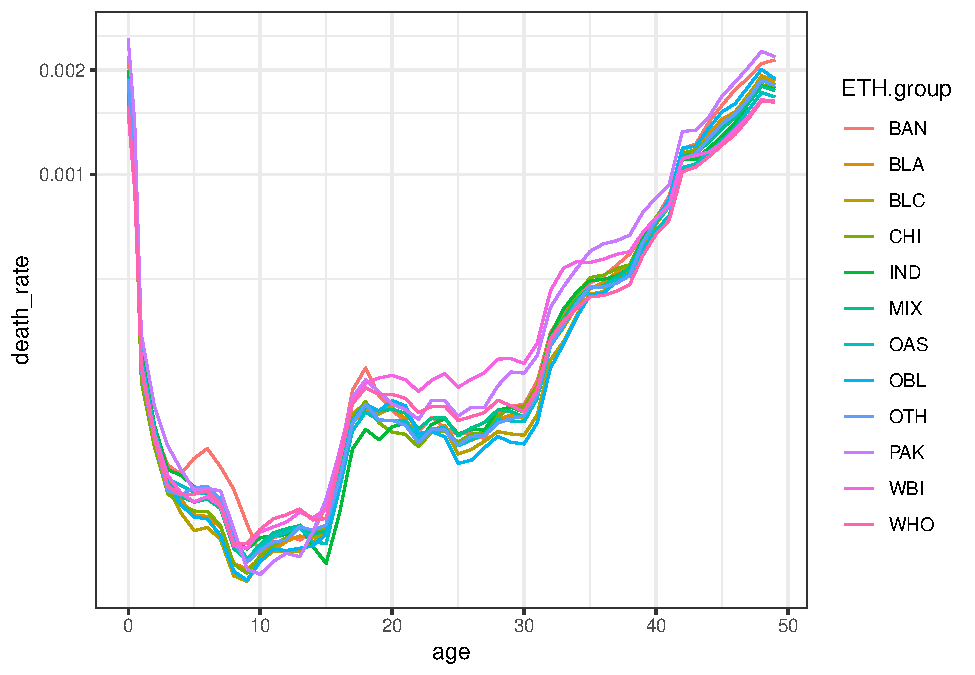
\includegraphics{C:/Users/Nathan/Documents/R/survivorETHPOP/docs/analysis_files/figure-latex/unnamed-chunk-5-1.pdf}

\begin{Shaded}
\begin{Highlighting}[]
\KeywordTok{ggplot}\NormalTok{(ETHPOP_lifetable_2011M, }\KeywordTok{aes}\NormalTok{(}\DataTypeTok{x =}\NormalTok{ age, }\DataTypeTok{y =}\NormalTok{ qx, }\DataTypeTok{colour =}\NormalTok{ ETH.group)) }\OperatorTok{+}
\StringTok{  }\KeywordTok{geom_line}\NormalTok{() }\OperatorTok{+}
\StringTok{  }\CommentTok{# scale_y_continuous(trans='log2') +}
\StringTok{  }\KeywordTok{coord_trans}\NormalTok{(}\DataTypeTok{y =} \StringTok{"log10"}\NormalTok{) }\OperatorTok{+}
\StringTok{  }\KeywordTok{theme_bw}\NormalTok{()}
\end{Highlighting}
\end{Shaded}

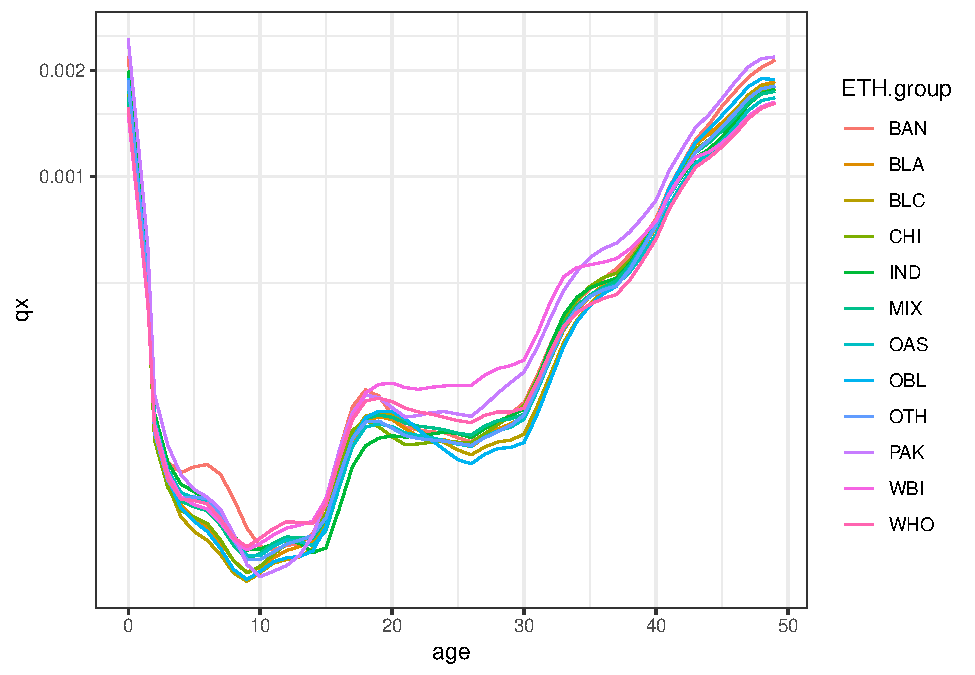
\includegraphics{C:/Users/Nathan/Documents/R/survivorETHPOP/docs/analysis_files/figure-latex/unnamed-chunk-5-2.pdf}

\begin{Shaded}
\begin{Highlighting}[]
\KeywordTok{ggplot}\NormalTok{(ETHPOP_lifetable_2011M, }\KeywordTok{aes}\NormalTok{(}\DataTypeTok{x =}\NormalTok{ age, }\DataTypeTok{y =}\NormalTok{ qx, }\DataTypeTok{colour =}\NormalTok{ ETH.group)) }\OperatorTok{+}
\StringTok{  }\KeywordTok{geom_line}\NormalTok{() }\OperatorTok{+}
\StringTok{  }\CommentTok{# scale_y_continuous(trans='log2') +}
\StringTok{  }\KeywordTok{theme_bw}\NormalTok{()}
\end{Highlighting}
\end{Shaded}

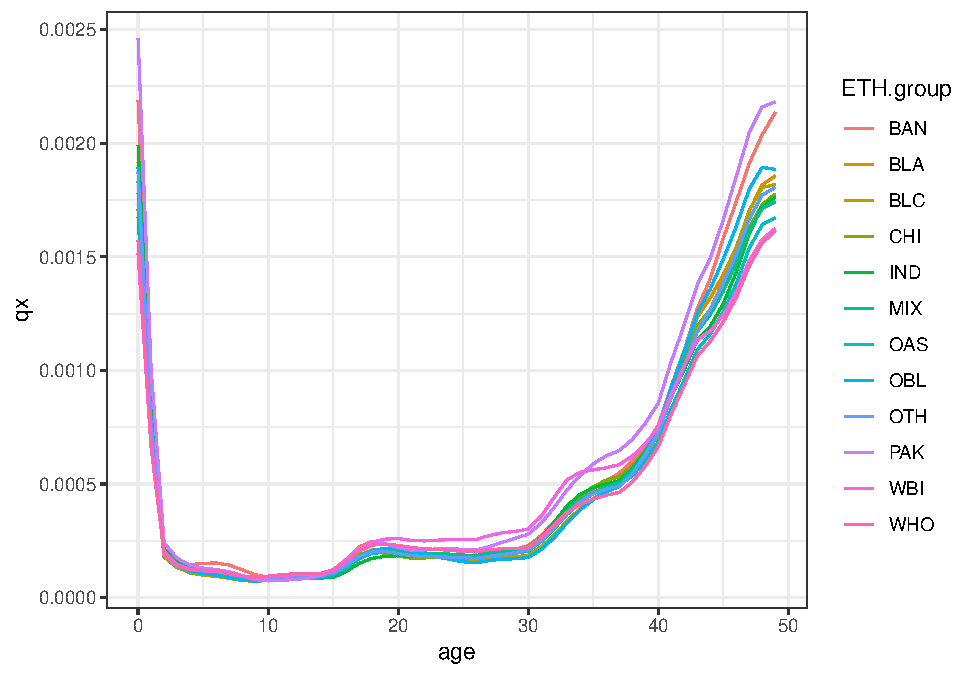
\includegraphics{C:/Users/Nathan/Documents/R/survivorETHPOP/docs/analysis_files/figure-latex/unnamed-chunk-5-3.pdf}

\begin{Shaded}
\begin{Highlighting}[]
\KeywordTok{ggplot}\NormalTok{(ETHPOP_lifetable_2011M, }\KeywordTok{aes}\NormalTok{(}\DataTypeTok{x =}\NormalTok{ age, }\DataTypeTok{y =}\NormalTok{ S, }\DataTypeTok{colour =}\NormalTok{ ETH.group)) }\OperatorTok{+}
\StringTok{  }\KeywordTok{geom_line}\NormalTok{() }\OperatorTok{+}
\StringTok{  }\KeywordTok{theme_bw}\NormalTok{()}
\end{Highlighting}
\end{Shaded}

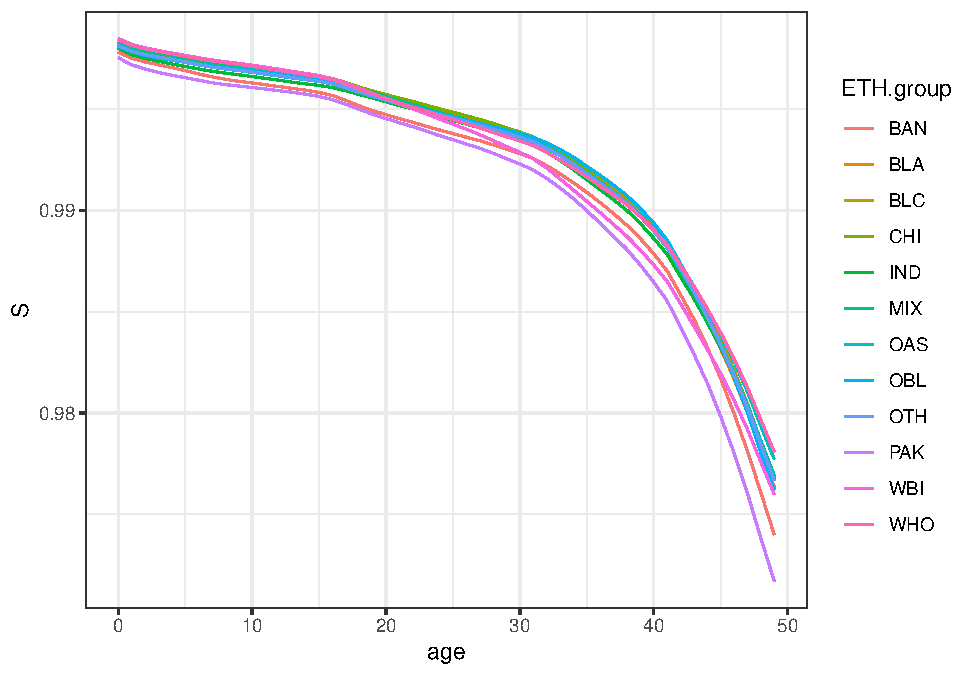
\includegraphics{C:/Users/Nathan/Documents/R/survivorETHPOP/docs/analysis_files/figure-latex/unnamed-chunk-5-4.pdf}

\begin{center}\rule{0.5\linewidth}{0.5pt}\end{center}

\hypertarget{ons-lifetables}{%
\section{ONS lifetables}\label{ons-lifetables}}

Read in and check.

\begin{Shaded}
\begin{Highlighting}[]
\NormalTok{lifetables <-}\StringTok{ }\KeywordTok{read_lifetables}\NormalTok{()}
\CommentTok{# save(lifetables, file = here::here("data", "lifetables.RData"))}


\NormalTok{ONS_lifetables <-}
\StringTok{  }\KeywordTok{do.call}\NormalTok{(rbind, lifetables) }\OperatorTok\StringTok{ }
\StringTok{  }\KeywordTok{mutate}\NormalTok{(}\DataTypeTok{new_yr =}\NormalTok{ year }\OperatorTok{<}\StringTok{ }\NormalTok{dplyr}\OperatorTok{::}\KeywordTok{lag}\NormalTok{(year, }\DataTypeTok{default =} \OtherTok{Inf}\NormalTok{),}
         \DataTypeTok{id =} \KeywordTok{cumsum}\NormalTok{(new_yr)) }\OperatorTok\StringTok{ }
\StringTok{  }\KeywordTok{group_by}\NormalTok{(id) }\OperatorTok\StringTok{ }
\StringTok{  }\KeywordTok{mutate}\NormalTok{(}\DataTypeTok{baseyr =} \KeywordTok{min}\NormalTok{(year)) }\OperatorTok\StringTok{ }
\StringTok{  }\KeywordTok{ungroup}\NormalTok{() }\OperatorTok\StringTok{ }
\StringTok{  }\KeywordTok{select}\NormalTok{(}\OperatorTok{-}\NormalTok{id, }\OperatorTok{-}\NormalTok{new_yr) }\OperatorTok\StringTok{ }
\StringTok{  }\KeywordTok{mutate}\NormalTok{(}\DataTypeTok{baseyr =} \KeywordTok{as.factor}\NormalTok{(baseyr))}
\end{Highlighting}
\end{Shaded}

\begin{Shaded}
\begin{Highlighting}[]
\KeywordTok{par}\NormalTok{(}\DataTypeTok{mfrow=} \KeywordTok{c}\NormalTok{(}\DecValTok{2}\NormalTok{,}\DecValTok{3}\NormalTok{))}
\ControlFlowTok{for}\NormalTok{ (i }\ControlFlowTok{in} \KeywordTok{seq_along}\NormalTok{(lifetables)) \{}
  \KeywordTok{plot}\NormalTok{(}\DataTypeTok{x =}\NormalTok{ lifetables[[i]]}\OperatorTok{$}\NormalTok{year[lifetables[[i]]}\OperatorTok{$}\NormalTok{sex }\OperatorTok{==}\StringTok{ "M"}\NormalTok{],}
       \DataTypeTok{y =}\NormalTok{ lifetables[[i]]}\OperatorTok{$}\NormalTok{qx[lifetables[[i]]}\OperatorTok{$}\NormalTok{sex }\OperatorTok{==}\StringTok{ "M"}\NormalTok{], }\DataTypeTok{log =} \StringTok{"y"}\NormalTok{, }\DataTypeTok{type =} \StringTok{"l"}\NormalTok{,}
       \DataTypeTok{main =} \KeywordTok{names}\NormalTok{(lifetables)[i], }\DataTypeTok{ylab =} \StringTok{"h"}\NormalTok{, }\DataTypeTok{xlab =} \StringTok{"year"}\NormalTok{)}
  \KeywordTok{lines}\NormalTok{(}\DataTypeTok{x =}\NormalTok{ lifetables[[i]]}\OperatorTok{$}\NormalTok{year[lifetables[[i]]}\OperatorTok{$}\NormalTok{sex }\OperatorTok{==}\StringTok{ "F"}\NormalTok{],}
        \DataTypeTok{y =}\NormalTok{ lifetables[[i]]}\OperatorTok{$}\NormalTok{qx[lifetables[[i]]}\OperatorTok{$}\NormalTok{sex }\OperatorTok{==}\StringTok{ "F"}\NormalTok{], }\DataTypeTok{log =} \StringTok{"y"}\NormalTok{, }\DataTypeTok{type =} \StringTok{"l"}\NormalTok{, }\DataTypeTok{col =} \StringTok{"red"}\NormalTok{)}
\NormalTok{\}}
\end{Highlighting}
\end{Shaded}

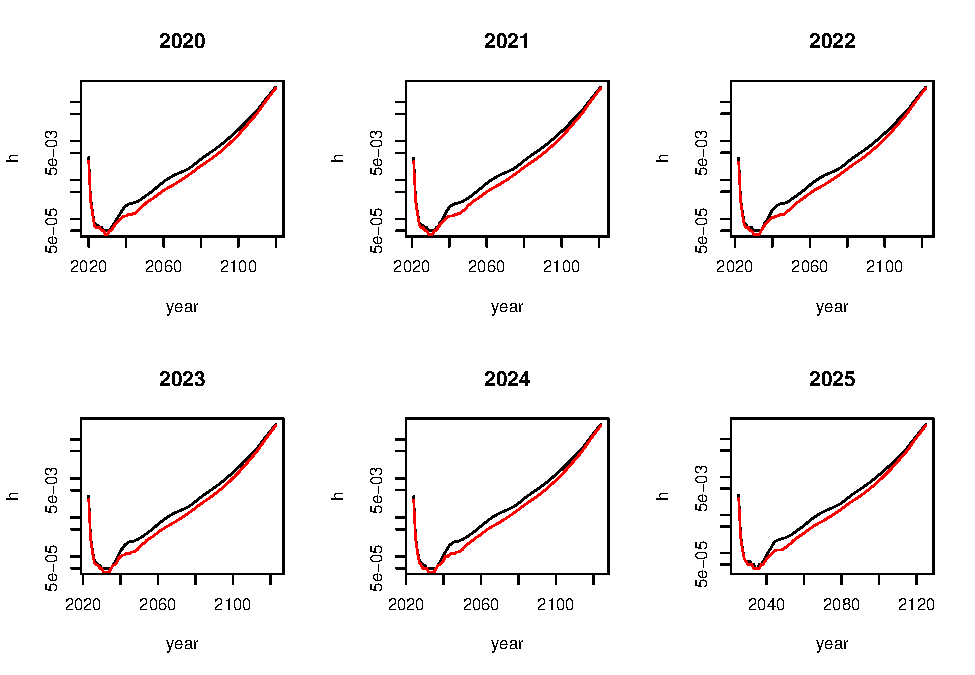
\includegraphics{C:/Users/Nathan/Documents/R/survivorETHPOP/docs/analysis_files/figure-latex/unnamed-chunk-7-1.pdf}
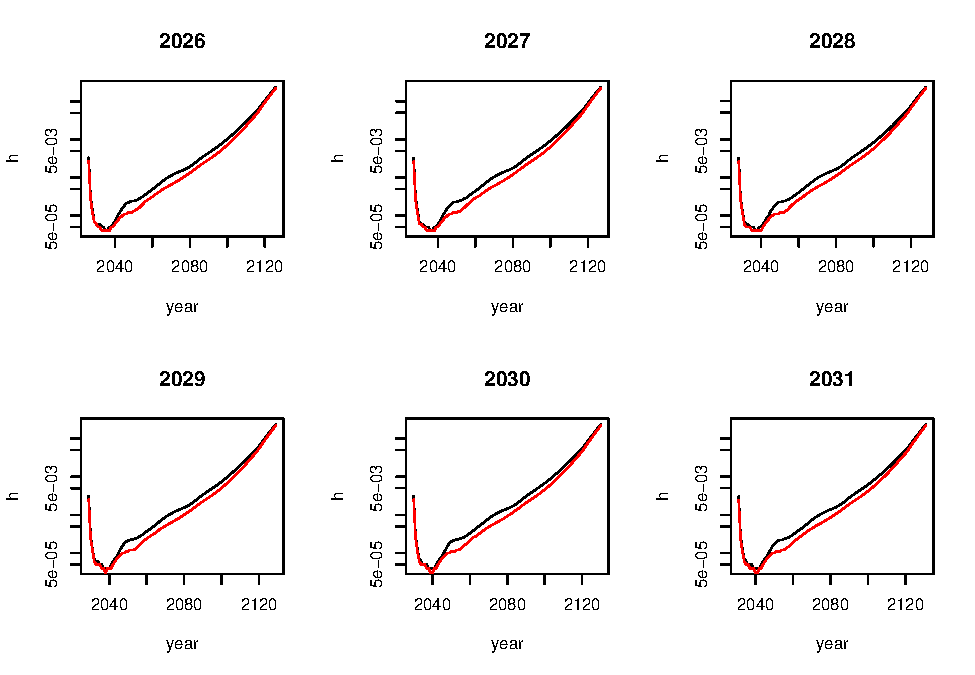
\includegraphics{C:/Users/Nathan/Documents/R/survivorETHPOP/docs/analysis_files/figure-latex/unnamed-chunk-7-2.pdf}
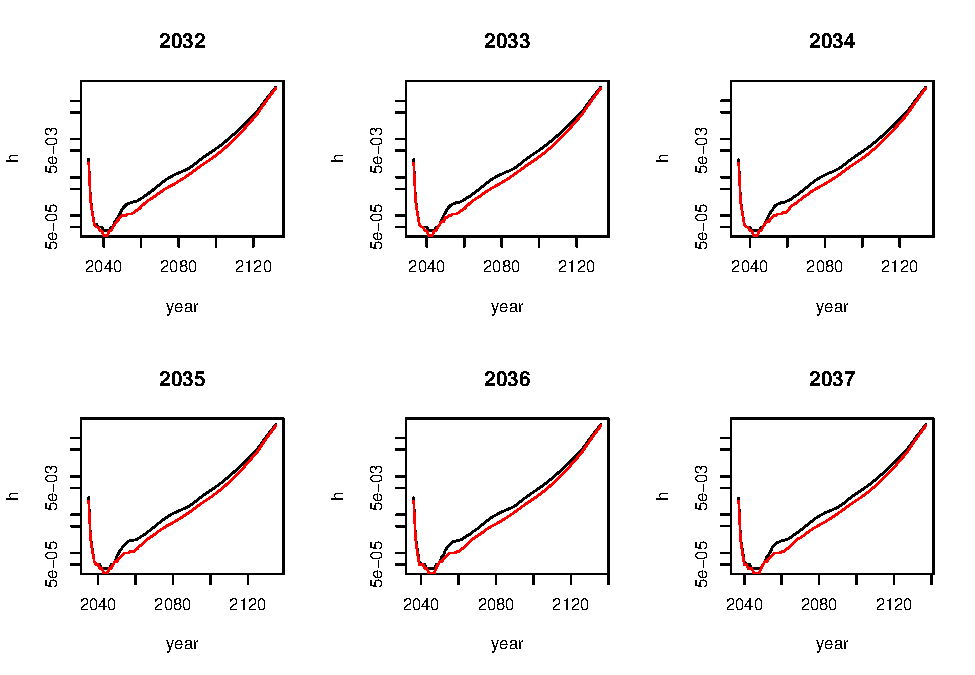
\includegraphics{C:/Users/Nathan/Documents/R/survivorETHPOP/docs/analysis_files/figure-latex/unnamed-chunk-7-3.pdf}

\begin{Shaded}
\begin{Highlighting}[]
\KeywordTok{par}\NormalTok{(}\DataTypeTok{mfrow=} \KeywordTok{c}\NormalTok{(}\DecValTok{1}\NormalTok{,}\DecValTok{2}\NormalTok{))}
\end{Highlighting}
\end{Shaded}

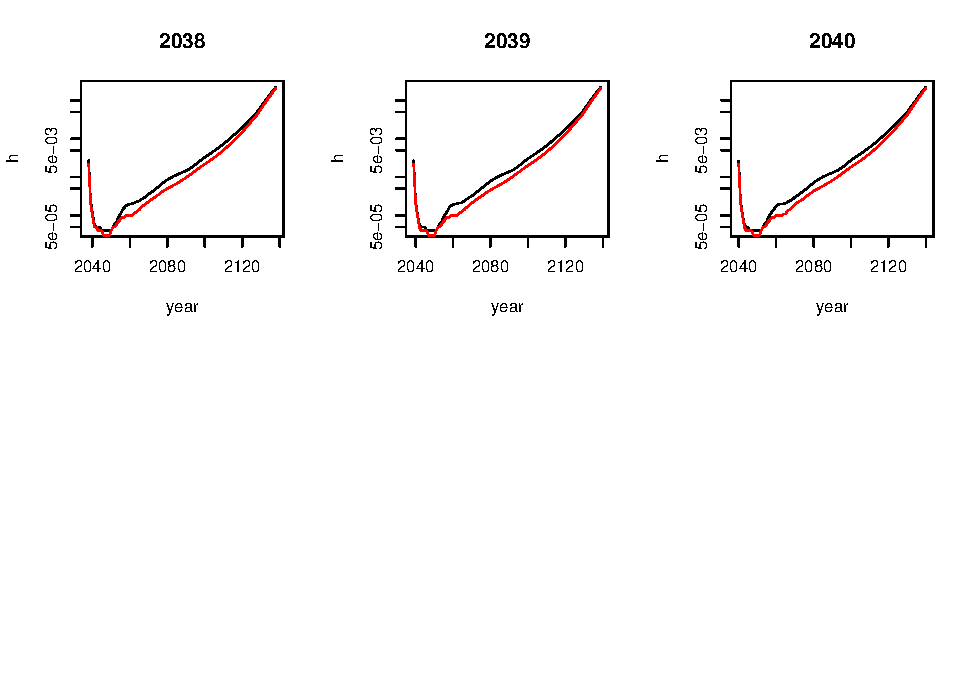
\includegraphics{C:/Users/Nathan/Documents/R/survivorETHPOP/docs/analysis_files/figure-latex/unnamed-chunk-7-4.pdf}

\begin{Shaded}
\begin{Highlighting}[]
\ControlFlowTok{for}\NormalTok{ (j }\ControlFlowTok{in} \KeywordTok{c}\NormalTok{(}\StringTok{"M"}\NormalTok{,}\StringTok{"F"}\NormalTok{)) \{}
  \KeywordTok{plot}\NormalTok{(}\DataTypeTok{x =}\NormalTok{ lifetables[[}\DecValTok{1}\NormalTok{]]}\OperatorTok{$}\NormalTok{age[lifetables[[}\DecValTok{1}\NormalTok{]]}\OperatorTok{$}\NormalTok{sex }\OperatorTok{==}\StringTok{ }\NormalTok{j],}
       \DataTypeTok{y =}\NormalTok{ lifetables[[}\DecValTok{1}\NormalTok{]]}\OperatorTok{$}\NormalTok{qx[lifetables[[}\DecValTok{1}\NormalTok{]]}\OperatorTok{$}\NormalTok{sex }\OperatorTok{==}\StringTok{ }\NormalTok{j], }\DataTypeTok{log =} \StringTok{"y"}\NormalTok{, }\DataTypeTok{type =} \StringTok{"l"}\NormalTok{,}
       \DataTypeTok{main =}\NormalTok{ j, }\DataTypeTok{ylab =} \StringTok{"h"}\NormalTok{, }\DataTypeTok{xlab =} \StringTok{"age"}\NormalTok{)}
  \ControlFlowTok{for}\NormalTok{ (i }\ControlFlowTok{in} \KeywordTok{seq_along}\NormalTok{(lifetables)) \{}
    \KeywordTok{lines}\NormalTok{(}\DataTypeTok{x =}\NormalTok{ lifetables[[i]]}\OperatorTok{$}\NormalTok{age[lifetables[[i]]}\OperatorTok{$}\NormalTok{sex }\OperatorTok{==}\StringTok{ }\NormalTok{j],}
          \DataTypeTok{y =}\NormalTok{ lifetables[[i]]}\OperatorTok{$}\NormalTok{qx[lifetables[[i]]}\OperatorTok{$}\NormalTok{sex }\OperatorTok{==}\StringTok{ }\NormalTok{j], }\DataTypeTok{log =} \StringTok{"y"}\NormalTok{, }\DataTypeTok{type =} \StringTok{"l"}\NormalTok{, }\DataTypeTok{col =}\NormalTok{ i)}
\NormalTok{  \}}
\NormalTok{\}}
\end{Highlighting}
\end{Shaded}

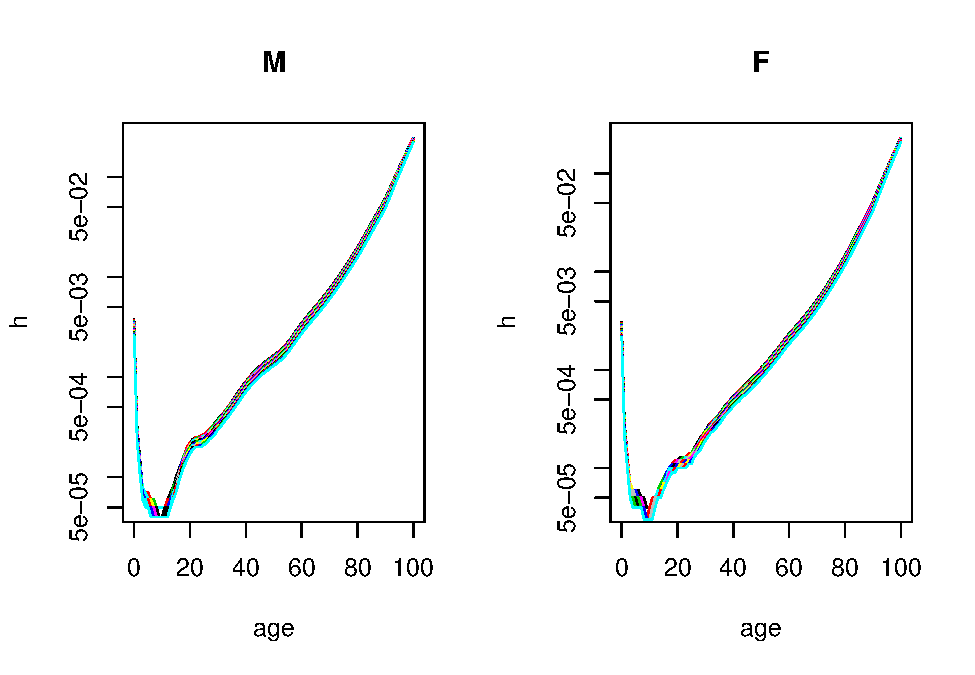
\includegraphics{C:/Users/Nathan/Documents/R/survivorETHPOP/docs/analysis_files/figure-latex/unnamed-chunk-7-5.pdf}

\begin{Shaded}
\begin{Highlighting}[]
\KeywordTok{ggplot}\NormalTok{(ONS_lifetables, }\KeywordTok{aes}\NormalTok{(}\DataTypeTok{x =}\NormalTok{ age, }\DataTypeTok{y =}\NormalTok{ qx, }\DataTypeTok{colour =} \KeywordTok{interaction}\NormalTok{(sex, baseyr))) }\OperatorTok{+}
\StringTok{  }\KeywordTok{geom_line}\NormalTok{() }\OperatorTok{+}
\StringTok{  }\CommentTok{# scale_y_continuous(trans='log2') +}
\StringTok{  }\KeywordTok{coord_trans}\NormalTok{(}\DataTypeTok{y =} \StringTok{"log10"}\NormalTok{) }\OperatorTok{+}
\StringTok{  }\KeywordTok{theme_bw}\NormalTok{()}
\end{Highlighting}
\end{Shaded}

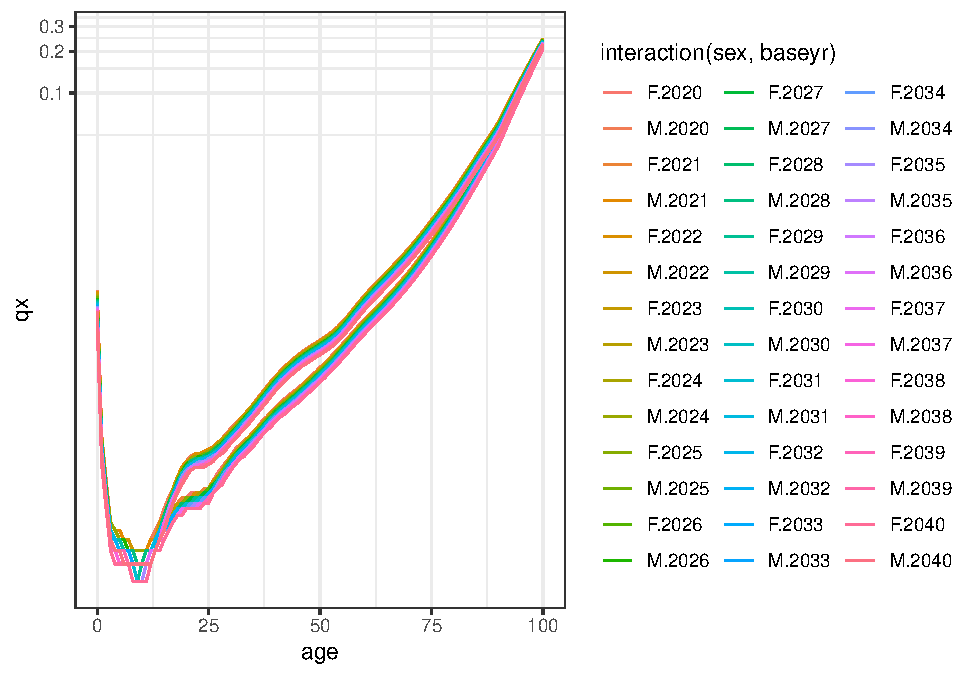
\includegraphics{C:/Users/Nathan/Documents/R/survivorETHPOP/docs/analysis_files/figure-latex/unnamed-chunk-8-1.pdf}

\hypertarget{comparison-with-ons-and-ethpop}{%
\section{Comparison with ONS and
ETHPOP}\label{comparison-with-ons-and-ethpop}}

2011

\begin{Shaded}
\begin{Highlighting}[]
\KeywordTok{ggplot}\NormalTok{(ETHPOP_lifetable_2011M, }\KeywordTok{aes}\NormalTok{(}\DataTypeTok{x =}\NormalTok{ age, }\DataTypeTok{y =}\NormalTok{ death_rate, }\DataTypeTok{colour =}\NormalTok{ ETH.group)) }\OperatorTok{+}
\StringTok{  }\KeywordTok{geom_line}\NormalTok{() }\OperatorTok{+}
\StringTok{  }\KeywordTok{coord_trans}\NormalTok{(}\DataTypeTok{y =} \StringTok{"log10"}\NormalTok{) }\OperatorTok{+}
\StringTok{  }\KeywordTok{ggtitle}\NormalTok{(}\StringTok{"Male 2011"}\NormalTok{) }\OperatorTok{+}
\StringTok{  }\KeywordTok{theme_bw}\NormalTok{() }\OperatorTok{+}
\StringTok{  }\KeywordTok{geom_line}\NormalTok{(}\KeywordTok{aes}\NormalTok{(age, qx, }\DataTypeTok{colour =} \StringTok{"ONS"}\NormalTok{),}
            \DataTypeTok{data =}\NormalTok{ ONS_lifetables[ONS_lifetables}\OperatorTok{$}\NormalTok{baseyr }\OperatorTok{==}\StringTok{ }\DecValTok{2011} \OperatorTok{&}\StringTok{ }\NormalTok{ONS_lifetables}\OperatorTok{$}\NormalTok{sex }\OperatorTok{==}\StringTok{ "M"}\NormalTok{, ],}
            \DataTypeTok{colour =} \StringTok{"black"}\NormalTok{)}
\end{Highlighting}
\end{Shaded}

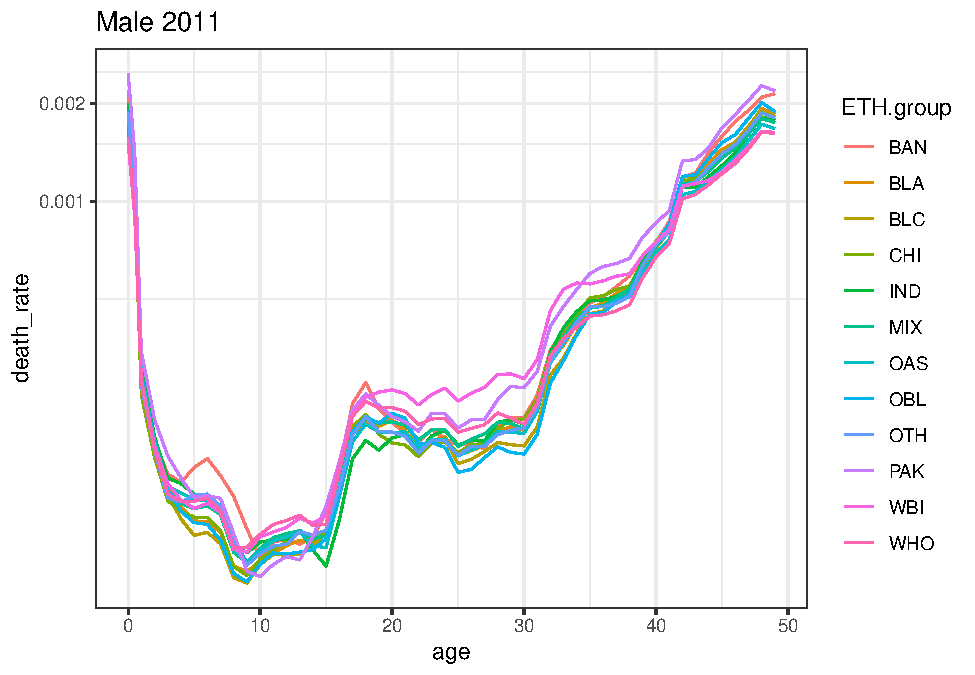
\includegraphics{C:/Users/Nathan/Documents/R/survivorETHPOP/docs/analysis_files/figure-latex/unnamed-chunk-9-1.pdf}

\begin{Shaded}
\begin{Highlighting}[]
\KeywordTok{ggplot}\NormalTok{(ETHPOP_lifetable_2011F, }\KeywordTok{aes}\NormalTok{(}\DataTypeTok{x =}\NormalTok{ age, }\DataTypeTok{y =}\NormalTok{ death_rate, }\DataTypeTok{colour =}\NormalTok{ ETH.group)) }\OperatorTok{+}
\StringTok{  }\KeywordTok{geom_line}\NormalTok{() }\OperatorTok{+}
\StringTok{  }\KeywordTok{ggtitle}\NormalTok{(}\StringTok{"Female 2011"}\NormalTok{) }\OperatorTok{+}
\StringTok{  }\KeywordTok{coord_trans}\NormalTok{(}\DataTypeTok{y =} \StringTok{"log10"}\NormalTok{) }\OperatorTok{+}
\StringTok{  }\KeywordTok{theme_bw}\NormalTok{() }\OperatorTok{+}
\StringTok{  }\KeywordTok{geom_line}\NormalTok{(}\KeywordTok{aes}\NormalTok{(age, qx, }\DataTypeTok{colour =} \StringTok{"ONS"}\NormalTok{),}
            \DataTypeTok{data =}\NormalTok{ ONS_lifetables[ONS_lifetables}\OperatorTok{$}\NormalTok{baseyr }\OperatorTok{==}\StringTok{ }\DecValTok{2011} \OperatorTok{&}\StringTok{ }\NormalTok{ONS_lifetables}\OperatorTok{$}\NormalTok{sex }\OperatorTok{==}\StringTok{ "F"}\NormalTok{, ],}
            \DataTypeTok{colour =} \StringTok{"black"}\NormalTok{)}
\end{Highlighting}
\end{Shaded}

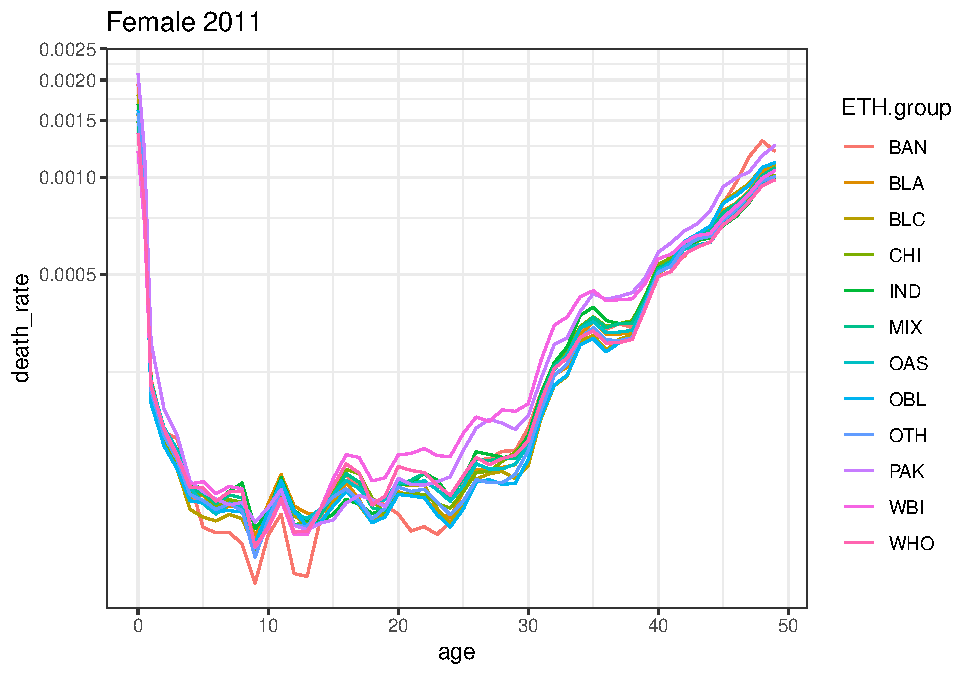
\includegraphics{C:/Users/Nathan/Documents/R/survivorETHPOP/docs/analysis_files/figure-latex/unnamed-chunk-9-2.pdf}

\begin{Shaded}
\begin{Highlighting}[]
\KeywordTok{ggplot}\NormalTok{(ETHPOP_lifetable_2011M, }\KeywordTok{aes}\NormalTok{(}\DataTypeTok{x =}\NormalTok{ age, }\DataTypeTok{y =}\NormalTok{ death_rate, }\DataTypeTok{colour =}\NormalTok{ ETH.group)) }\OperatorTok{+}
\StringTok{  }\KeywordTok{geom_line}\NormalTok{() }\OperatorTok{+}
\StringTok{  }\KeywordTok{ggtitle}\NormalTok{(}\StringTok{"Male 2011"}\NormalTok{) }\OperatorTok{+}
\StringTok{  }\KeywordTok{theme_bw}\NormalTok{() }\OperatorTok{+}
\StringTok{  }\KeywordTok{geom_line}\NormalTok{(}\KeywordTok{aes}\NormalTok{(age, qx, }\DataTypeTok{colour =} \StringTok{"ONS"}\NormalTok{),}
            \DataTypeTok{data =}\NormalTok{ ONS_lifetables[ONS_lifetables}\OperatorTok{$}\NormalTok{baseyr }\OperatorTok{==}\StringTok{ }\DecValTok{2011} \OperatorTok{&}\StringTok{ }\NormalTok{ONS_lifetables}\OperatorTok{$}\NormalTok{sex }\OperatorTok{==}\StringTok{ "M"}\NormalTok{, ],}
            \DataTypeTok{colour =} \StringTok{"black"}\NormalTok{) }\OperatorTok{+}
\StringTok{  }\KeywordTok{ylim}\NormalTok{(}\DecValTok{0}\NormalTok{, }\FloatTok{0.003}\NormalTok{) }\OperatorTok{+}\StringTok{ }\KeywordTok{xlim}\NormalTok{(}\DecValTok{0}\NormalTok{, }\DecValTok{60}\NormalTok{)}
\end{Highlighting}
\end{Shaded}

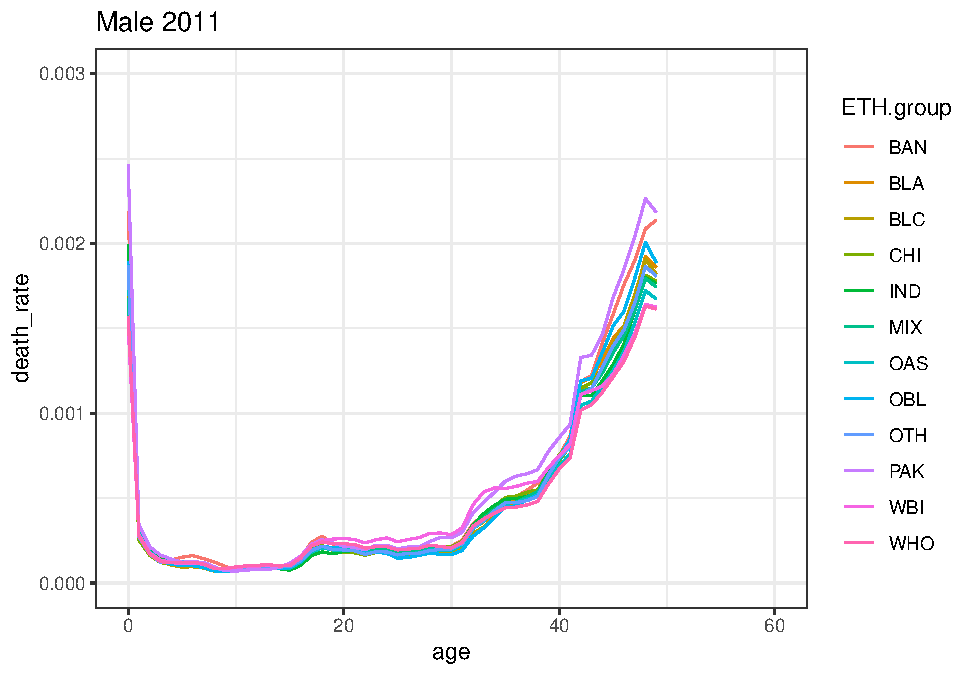
\includegraphics{C:/Users/Nathan/Documents/R/survivorETHPOP/docs/analysis_files/figure-latex/unnamed-chunk-10-1.pdf}

\begin{Shaded}
\begin{Highlighting}[]
\KeywordTok{ggplot}\NormalTok{(ETHPOP_lifetable_2011F, }\KeywordTok{aes}\NormalTok{(}\DataTypeTok{x =}\NormalTok{ age, }\DataTypeTok{y =}\NormalTok{ death_rate, }\DataTypeTok{colour =}\NormalTok{ ETH.group)) }\OperatorTok{+}
\StringTok{  }\KeywordTok{geom_line}\NormalTok{() }\OperatorTok{+}
\StringTok{  }\KeywordTok{ggtitle}\NormalTok{(}\StringTok{"Female 2011"}\NormalTok{) }\OperatorTok{+}
\StringTok{  }\KeywordTok{theme_bw}\NormalTok{() }\OperatorTok{+}
\StringTok{  }\KeywordTok{geom_line}\NormalTok{(}\KeywordTok{aes}\NormalTok{(age, qx, }\DataTypeTok{colour =} \StringTok{"ONS"}\NormalTok{),}
            \DataTypeTok{data =}\NormalTok{ ONS_lifetables[ONS_lifetables}\OperatorTok{$}\NormalTok{baseyr }\OperatorTok{==}\StringTok{ }\DecValTok{2011} \OperatorTok{&}\StringTok{ }\NormalTok{ONS_lifetables}\OperatorTok{$}\NormalTok{sex }\OperatorTok{==}\StringTok{ "F"}\NormalTok{, ],}
            \DataTypeTok{colour =} \StringTok{"black"}\NormalTok{) }\OperatorTok{+}
\StringTok{  }\KeywordTok{ylim}\NormalTok{(}\DecValTok{0}\NormalTok{, }\FloatTok{0.003}\NormalTok{) }\OperatorTok{+}\StringTok{ }\KeywordTok{xlim}\NormalTok{(}\DecValTok{0}\NormalTok{, }\DecValTok{60}\NormalTok{)}
\end{Highlighting}
\end{Shaded}

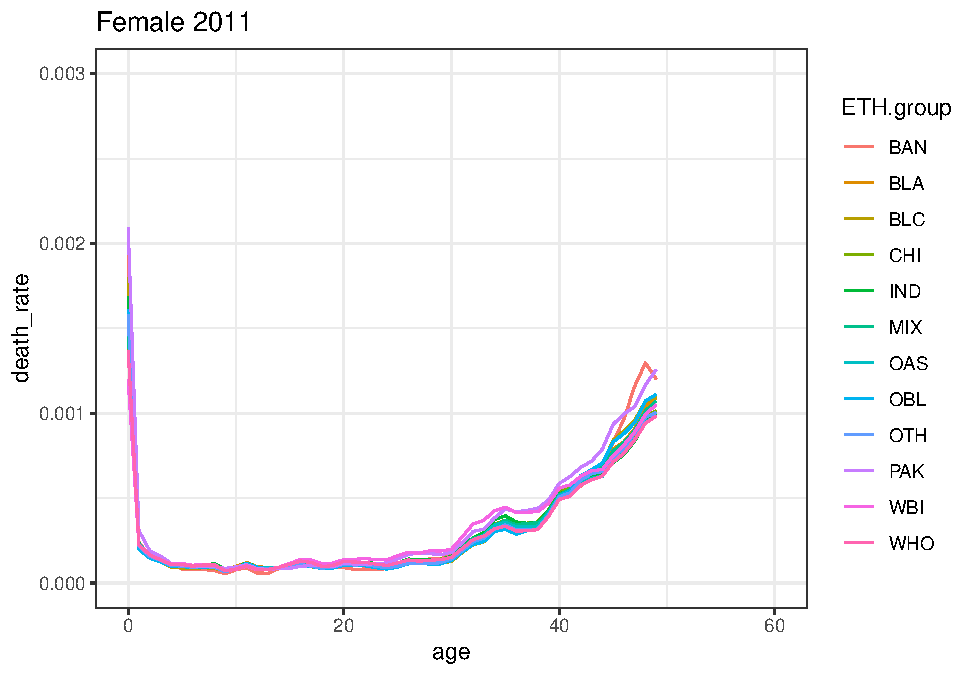
\includegraphics{C:/Users/Nathan/Documents/R/survivorETHPOP/docs/analysis_files/figure-latex/unnamed-chunk-10-2.pdf}

2030

\begin{Shaded}
\begin{Highlighting}[]
\NormalTok{baseyr_}\DecValTok{2030}\NormalTok{ <-}\StringTok{ }\NormalTok{ETHPOP_lifetable}\OperatorTok{$}\NormalTok{id[ETHPOP_lifetable}\OperatorTok{$}\NormalTok{yr_age }\OperatorTok{==}\StringTok{ "2030_0"}\NormalTok{][}\DecValTok{1}\NormalTok{]}

\NormalTok{ETHPOP_lifetable[ETHPOP_lifetable}\OperatorTok{$}\NormalTok{id }\OperatorTok{==}\StringTok{ }\NormalTok{baseyr_}\DecValTok{2030} \OperatorTok{&}\StringTok{ }\NormalTok{ETHPOP_lifetable}\OperatorTok{$}\NormalTok{sex }\OperatorTok{==}\StringTok{ "M"}\NormalTok{, ] }\OperatorTok\StringTok{ }
\StringTok{  }\KeywordTok{ggplot}\NormalTok{(}\KeywordTok{aes}\NormalTok{(}\DataTypeTok{x =}\NormalTok{ age, }\DataTypeTok{y =}\NormalTok{ death_rate, }\DataTypeTok{colour =}\NormalTok{ ETH.group)) }\OperatorTok{+}
\StringTok{  }\KeywordTok{geom_line}\NormalTok{() }\OperatorTok{+}
\StringTok{  }\KeywordTok{coord_trans}\NormalTok{(}\DataTypeTok{y =} \StringTok{"log10"}\NormalTok{) }\OperatorTok{+}
\StringTok{  }\KeywordTok{ggtitle}\NormalTok{(}\StringTok{"Male 2030"}\NormalTok{) }\OperatorTok{+}
\StringTok{  }\KeywordTok{theme_bw}\NormalTok{() }\OperatorTok{+}
\StringTok{  }\KeywordTok{geom_line}\NormalTok{(}\KeywordTok{aes}\NormalTok{(age, qx, }\DataTypeTok{colour =} \StringTok{"ONS"}\NormalTok{),}
            \DataTypeTok{data =}\NormalTok{ ONS_lifetables[ONS_lifetables}\OperatorTok{$}\NormalTok{baseyr }\OperatorTok{==}\StringTok{ }\DecValTok{2030} \OperatorTok{&}\StringTok{ }\NormalTok{ONS_lifetables}\OperatorTok{$}\NormalTok{sex }\OperatorTok{==}\StringTok{ "M"}\NormalTok{, ],}
            \DataTypeTok{colour =} \StringTok{"black"}\NormalTok{)}
\end{Highlighting}
\end{Shaded}

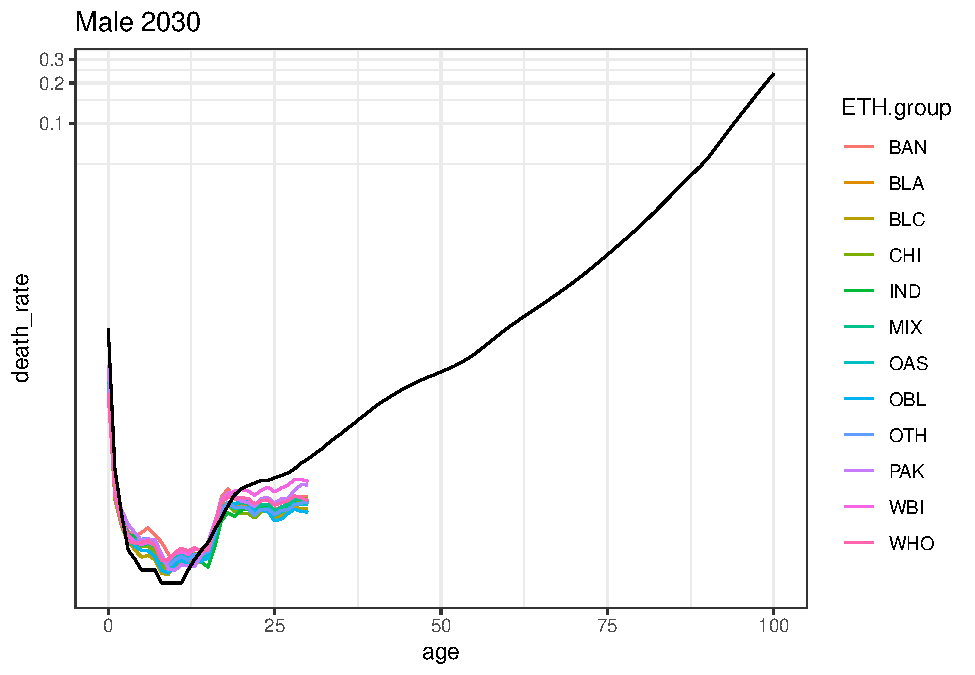
\includegraphics{C:/Users/Nathan/Documents/R/survivorETHPOP/docs/analysis_files/figure-latex/unnamed-chunk-11-1.pdf}

\begin{Shaded}
\begin{Highlighting}[]
\NormalTok{ETHPOP_lifetable[ETHPOP_lifetable}\OperatorTok{$}\NormalTok{id }\OperatorTok{==}\StringTok{ }\NormalTok{baseyr_}\DecValTok{2030} \OperatorTok{&}\StringTok{ }\NormalTok{ETHPOP_lifetable}\OperatorTok{$}\NormalTok{sex }\OperatorTok{==}\StringTok{ "F"}\NormalTok{, ] }\OperatorTok\StringTok{ }
\StringTok{  }\KeywordTok{ggplot}\NormalTok{(}\KeywordTok{aes}\NormalTok{(}\DataTypeTok{x =}\NormalTok{ age, }\DataTypeTok{y =}\NormalTok{ death_rate, }\DataTypeTok{colour =}\NormalTok{ ETH.group)) }\OperatorTok{+}
\StringTok{  }\KeywordTok{geom_line}\NormalTok{() }\OperatorTok{+}
\StringTok{  }\KeywordTok{ggtitle}\NormalTok{(}\StringTok{"Female 2030"}\NormalTok{) }\OperatorTok{+}
\StringTok{  }\KeywordTok{coord_trans}\NormalTok{(}\DataTypeTok{y =} \StringTok{"log10"}\NormalTok{) }\OperatorTok{+}
\StringTok{  }\KeywordTok{theme_bw}\NormalTok{() }\OperatorTok{+}
\StringTok{  }\KeywordTok{geom_line}\NormalTok{(}\KeywordTok{aes}\NormalTok{(age, qx, }\DataTypeTok{colour =} \StringTok{"ONS"}\NormalTok{),}
            \DataTypeTok{data =}\NormalTok{ ONS_lifetables[ONS_lifetables}\OperatorTok{$}\NormalTok{baseyr }\OperatorTok{==}\StringTok{ }\DecValTok{2030} \OperatorTok{&}\StringTok{ }\NormalTok{ONS_lifetables}\OperatorTok{$}\NormalTok{sex }\OperatorTok{==}\StringTok{ "F"}\NormalTok{, ],}
            \DataTypeTok{colour =} \StringTok{"black"}\NormalTok{)}
\end{Highlighting}
\end{Shaded}

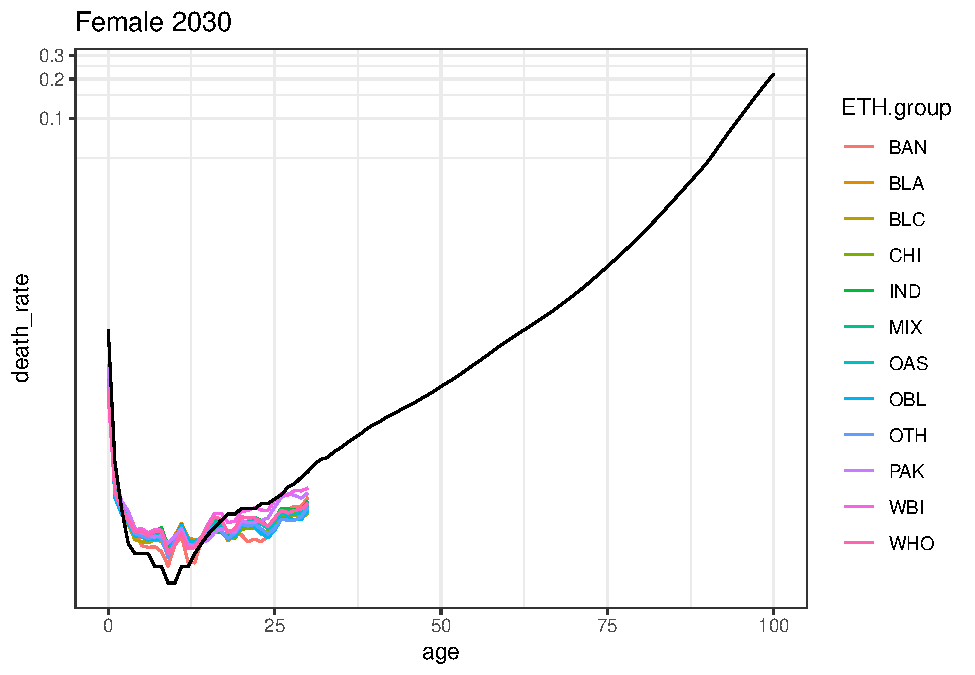
\includegraphics{C:/Users/Nathan/Documents/R/survivorETHPOP/docs/analysis_files/figure-latex/unnamed-chunk-11-2.pdf}

\begin{Shaded}
\begin{Highlighting}[]
\NormalTok{baseyr_}\DecValTok{2030}\NormalTok{ <-}\StringTok{ }\NormalTok{ETHPOP_lifetable}\OperatorTok{$}\NormalTok{id[ETHPOP_lifetable}\OperatorTok{$}\NormalTok{yr_age }\OperatorTok{==}\StringTok{ "2030_0"}\NormalTok{][}\DecValTok{1}\NormalTok{]}

\NormalTok{ETHPOP_lifetable[ETHPOP_lifetable}\OperatorTok{$}\NormalTok{id }\OperatorTok{==}\StringTok{ }\NormalTok{baseyr_}\DecValTok{2030} \OperatorTok{&}\StringTok{ }\NormalTok{ETHPOP_lifetable}\OperatorTok{$}\NormalTok{sex }\OperatorTok{==}\StringTok{ "M"}\NormalTok{, ] }\OperatorTok\StringTok{ }
\StringTok{  }\KeywordTok{ggplot}\NormalTok{(}\KeywordTok{aes}\NormalTok{(}\DataTypeTok{x =}\NormalTok{ age, }\DataTypeTok{y =}\NormalTok{ death_rate, }\DataTypeTok{colour =}\NormalTok{ ETH.group)) }\OperatorTok{+}
\StringTok{  }\KeywordTok{geom_line}\NormalTok{() }\OperatorTok{+}
\StringTok{  }\KeywordTok{ggtitle}\NormalTok{(}\StringTok{"Male 2030"}\NormalTok{) }\OperatorTok{+}
\StringTok{  }\KeywordTok{theme_bw}\NormalTok{() }\OperatorTok{+}
\StringTok{  }\KeywordTok{geom_line}\NormalTok{(}\KeywordTok{aes}\NormalTok{(age, qx, }\DataTypeTok{colour =} \StringTok{"ONS"}\NormalTok{),}
            \DataTypeTok{data =}\NormalTok{ ONS_lifetables[ONS_lifetables}\OperatorTok{$}\NormalTok{baseyr }\OperatorTok{==}\StringTok{ }\DecValTok{2030} \OperatorTok{&}\StringTok{ }\NormalTok{ONS_lifetables}\OperatorTok{$}\NormalTok{sex }\OperatorTok{==}\StringTok{ "M"}\NormalTok{, ],}
            \DataTypeTok{colour =} \StringTok{"black"}\NormalTok{) }\OperatorTok{+}
\StringTok{  }\KeywordTok{ylim}\NormalTok{(}\DecValTok{0}\NormalTok{, }\FloatTok{0.003}\NormalTok{) }\OperatorTok{+}\StringTok{ }\KeywordTok{xlim}\NormalTok{(}\DecValTok{0}\NormalTok{, }\DecValTok{40}\NormalTok{)}
\end{Highlighting}
\end{Shaded}

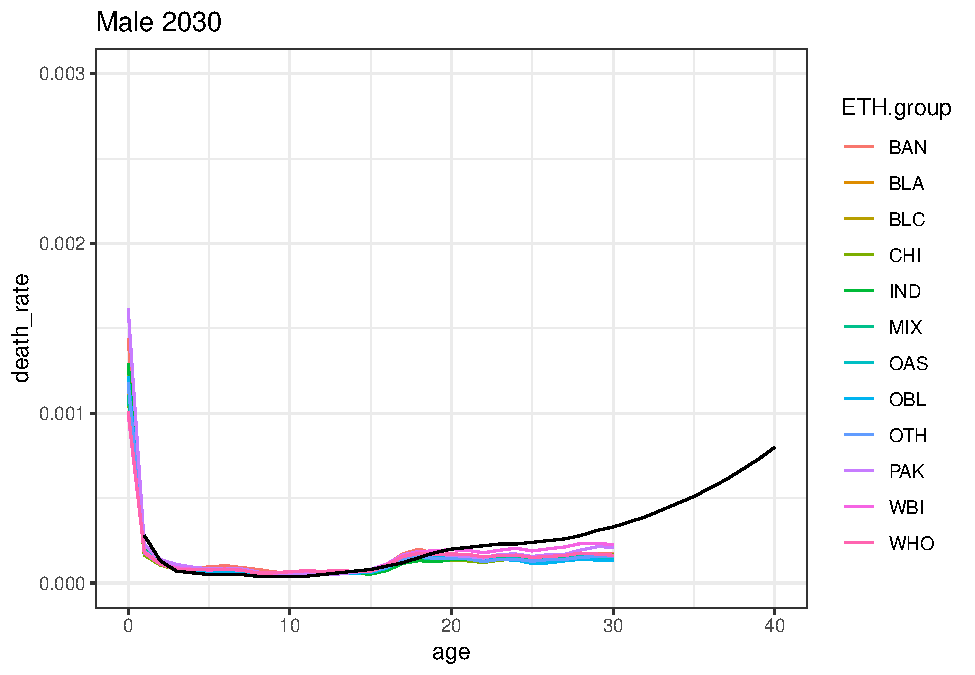
\includegraphics{C:/Users/Nathan/Documents/R/survivorETHPOP/docs/analysis_files/figure-latex/unnamed-chunk-12-1.pdf}

\begin{Shaded}
\begin{Highlighting}[]
\NormalTok{ETHPOP_lifetable[ETHPOP_lifetable}\OperatorTok{$}\NormalTok{id }\OperatorTok{==}\StringTok{ }\NormalTok{baseyr_}\DecValTok{2030} \OperatorTok{&}\StringTok{ }\NormalTok{ETHPOP_lifetable}\OperatorTok{$}\NormalTok{sex }\OperatorTok{==}\StringTok{ "F"}\NormalTok{, ] }\OperatorTok\StringTok{ }
\StringTok{  }\KeywordTok{ggplot}\NormalTok{(}\KeywordTok{aes}\NormalTok{(}\DataTypeTok{x =}\NormalTok{ age, }\DataTypeTok{y =}\NormalTok{ death_rate, }\DataTypeTok{colour =}\NormalTok{ ETH.group)) }\OperatorTok{+}
\StringTok{  }\KeywordTok{geom_line}\NormalTok{() }\OperatorTok{+}
\StringTok{  }\KeywordTok{ggtitle}\NormalTok{(}\StringTok{"Female 2030"}\NormalTok{) }\OperatorTok{+}
\StringTok{  }\KeywordTok{theme_bw}\NormalTok{() }\OperatorTok{+}
\StringTok{  }\KeywordTok{geom_line}\NormalTok{(}\KeywordTok{aes}\NormalTok{(age, qx, }\DataTypeTok{colour =} \StringTok{"ONS"}\NormalTok{),}
            \DataTypeTok{data =}\NormalTok{ ONS_lifetables[ONS_lifetables}\OperatorTok{$}\NormalTok{baseyr }\OperatorTok{==}\StringTok{ }\DecValTok{2030} \OperatorTok{&}\StringTok{ }\NormalTok{ONS_lifetables}\OperatorTok{$}\NormalTok{sex }\OperatorTok{==}\StringTok{ "F"}\NormalTok{, ],}
            \DataTypeTok{colour =} \StringTok{"black"}\NormalTok{) }\OperatorTok{+}
\StringTok{  }\KeywordTok{ylim}\NormalTok{(}\DecValTok{0}\NormalTok{, }\FloatTok{0.003}\NormalTok{) }\OperatorTok{+}\StringTok{ }\KeywordTok{xlim}\NormalTok{(}\DecValTok{0}\NormalTok{, }\DecValTok{40}\NormalTok{)}
\end{Highlighting}
\end{Shaded}

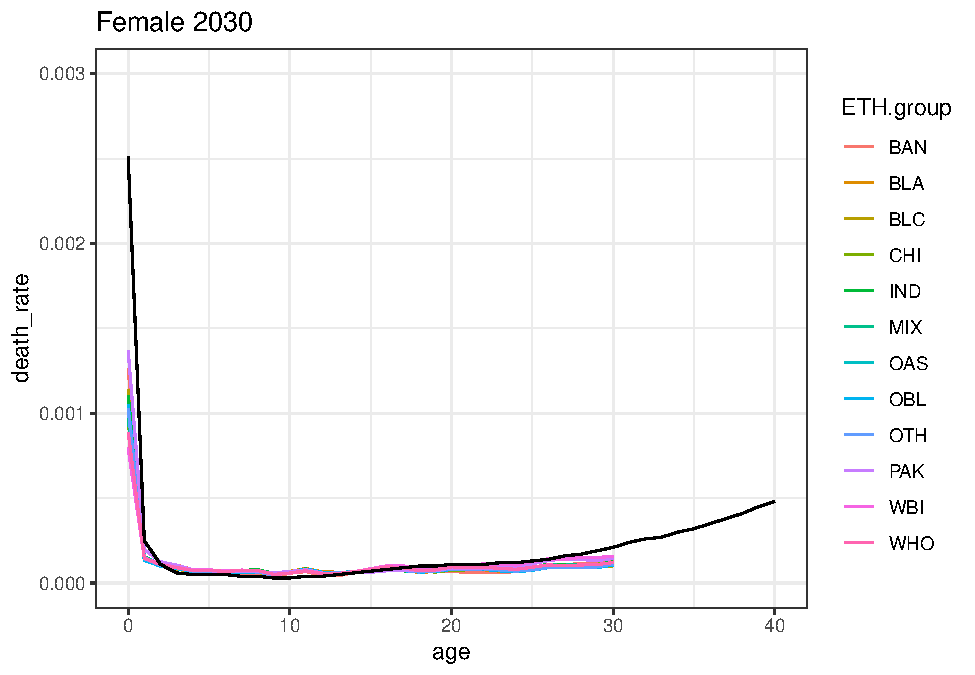
\includegraphics{C:/Users/Nathan/Documents/R/survivorETHPOP/docs/analysis_files/figure-latex/unnamed-chunk-12-2.pdf}

\hypertarget{life-expectancy}{%
\subsection{Life expectancy}\label{life-expectancy}}

ONS

\begin{Shaded}
\begin{Highlighting}[]
\KeywordTok{ggplot}\NormalTok{(ONS_lifetables[ONS_lifetables}\OperatorTok{$}\NormalTok{sex }\OperatorTok{==}\StringTok{ "M"}\NormalTok{, ], }\KeywordTok{aes}\NormalTok{(age, ex, }\DataTypeTok{colour =}\NormalTok{ baseyr)) }\OperatorTok{+}
\StringTok{  }\KeywordTok{geom_line}\NormalTok{() }\OperatorTok{+}
\StringTok{  }\KeywordTok{theme_bw}\NormalTok{()}
\end{Highlighting}
\end{Shaded}

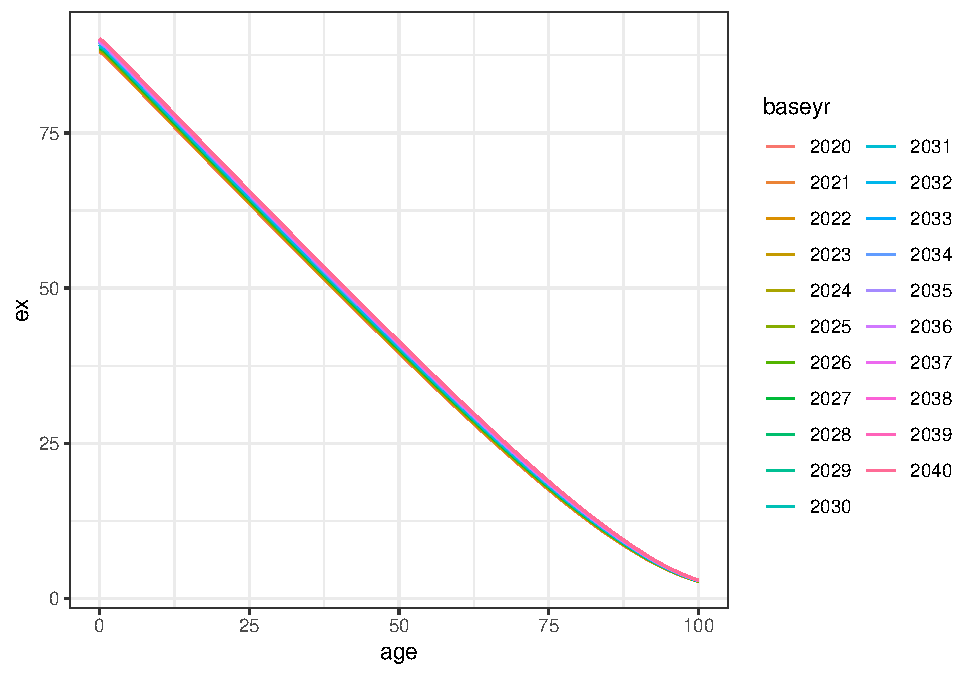
\includegraphics{C:/Users/Nathan/Documents/R/survivorETHPOP/docs/analysis_files/figure-latex/unnamed-chunk-13-1.pdf}

\begin{Shaded}
\begin{Highlighting}[]
\KeywordTok{ggplot}\NormalTok{(ONS_lifetables[ONS_lifetables}\OperatorTok{$}\NormalTok{sex }\OperatorTok{==}\StringTok{ "F"}\NormalTok{, ], }\KeywordTok{aes}\NormalTok{(age, ex, }\DataTypeTok{colour =}\NormalTok{ baseyr)) }\OperatorTok{+}
\StringTok{  }\KeywordTok{geom_line}\NormalTok{() }\OperatorTok{+}
\StringTok{  }\KeywordTok{theme_bw}\NormalTok{()}
\end{Highlighting}
\end{Shaded}

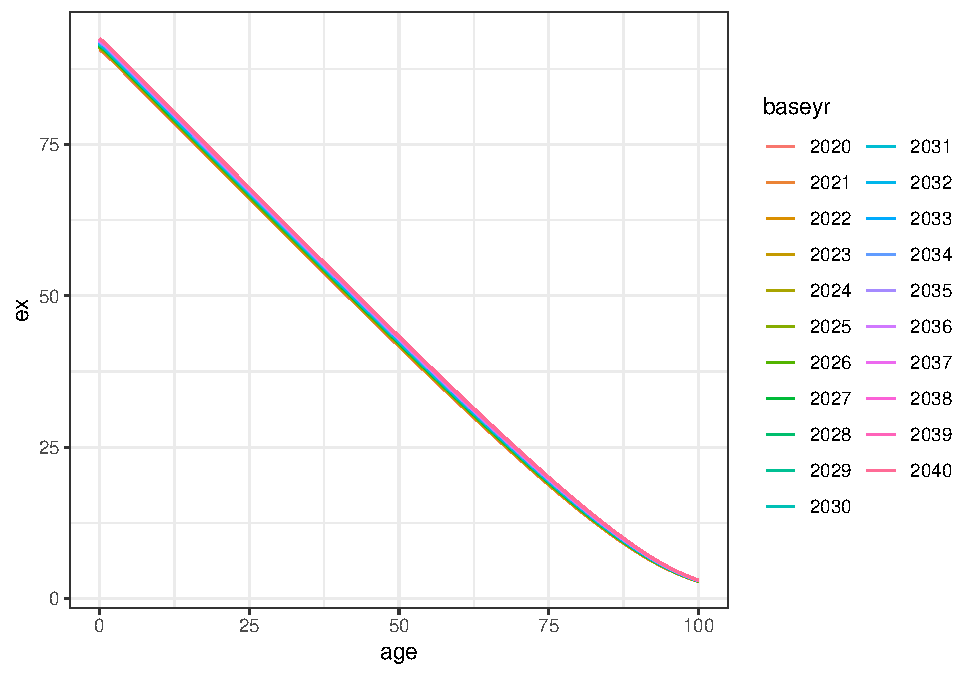
\includegraphics{C:/Users/Nathan/Documents/R/survivorETHPOP/docs/analysis_files/figure-latex/unnamed-chunk-13-2.pdf}

\end{document}
